\title{\textbf{LEKAv2: Linear-Time Efficient Kernel Attention with Landmark Distillation}}

\author{Anonymous authors}


\section{Introduction}

\subsection{Motivation}

Long-context inference is dominated by attention's $\mathcal{O}(L^2)$ cost. 
\textbf{Linear attention} (Katharopoulos et al., 2020) reduces this to 
$\mathcal{O}(L)$ via a kernel feature map $\phi$:

\[
\text{Attn}(Q, K, V) \approx \frac{\phi(Q)(\phi(K)^\top V)}{\phi(Q)(\phi(K)^\top \mathbf{1})}
\tag{1.1}
\]

However, linear attention has two limitations:

\begin{enumerate}
\item \textbf{Uniform aggregation.} The KV state $\phi(K)^\top V$ is a single global
  summary. Queries cannot selectively attend to specific tokens -- they
  only see the aggregate.
\item \textbf{Kernel approximation error.} RFF with $F$ features gives $\mathcal{O}(1/F)$
  approximation error; small $F$ degrades accuracy.

\end{enumerate}
\textbf{LEKAv1} (companion work) addressed the second via QR-orthogonalized 
projections. \textbf{LEKAv2} additionally addresses the first.

\subsection{Problem Statement}

Given $X \in \mathbb{R}^{B \times L \times d}$, we seek a hybrid attention 
that:

\begin{enumerate}
\item \textbf{Scales linearly} in $L$.
\item \textbf{Retains selective focus} on important tokens.
\item \textbf{Approximates a smooth kernel} (Gaussian RBF).
\item \textbf{Handles masking} without NaN or uniform collapse.
\item \textbf{Transfers pretrained weights} zero-shot.

\end{enumerate}
\subsection{Our Approach: LEKAv2}

LEKAv2 combines four components:

\subsubsection{Dual-Scale Random Features}

Two independent RFF projections with dimensions $F$ and $F/2$:

\[
\phi(x) = \frac{1}{\sqrt{F}} [\cos(x W_1) \| \sin(x W_1)] 
\| \frac{1}{\sqrt{F/2}} [\cos(x W_2) \| \sin(x W_2)]
\tag{1.2}
\]

with $W_1 \in \mathbb{R}^{d_h \times F}$, $W_2 \in \mathbb{R}^{d_h \times F/2}$.

\subsubsection{Landmark Distillation}

A learned scorer $s_\theta$ selects $L_\text{max} = \min(\rho L, L)$ 
landmark tokens:

\[
\mathcal{L}_\text{idx} = \text{TopK}(s_\theta(\phi(K)), L_\text{max})
\tag{1.3}
\]

Position 0 (\texttt{[CLS]}) is always retained.

\subsubsection{Softpick}

A ReLU-damped softmax that handles masked rows gracefully:

\[
\text{softpick}(x)_i = \frac{\text{ReLU}(e^{(x_i - m)/T} - e^{-m/T})}{\sum_j \text{ReLU}(e^{(x_j - m)/T} - e^{-m/T})}
\tag{1.4}
\]

with fallback to uniform when all entries are zero.

\subsubsection{Local-Global Fusion}

A per-head learnable gate blends local sliding-window attention and 
global landmark attention:

\[
\text{out} = (1 - g) \cdot \text{Local} + g \cdot \text{Global}, \quad g = \sigma(w_h)
\tag{1.5}
\]

with $w_h = -2$ initially, biasing toward local attention.

\subsection{Contributions}

\begin{itemize}
\item \textbf{Dual-scale RFF.} We extend RFF with a second projection at $F/2$,
  enriching the kernel representation.
\item \textbf{Learned landmark distillation.} A small scorer selects landmarks
  whose features are used in the global branch.
\item \textbf{Softpick.} A masked-attention-stable variant of softmax.
\item \textbf{Local-global fusion.} Per-head gate blends local and global paths.
\item \textbf{Per-head correction matrix.} $W_\text{corr} \in \mathbb{R}^{H \times d_h \times d_h}$
  applied to landmark values.
\item \textbf{Multi-architecture support.} DistilBERT, RoBERTa, GPT-2, Qwen3.5
  with GQA and RoPE.
\item \textbf{An honest evaluation.} We report both accuracy and parameter cost.

\end{itemize}
\subsection{Paper Organization}

Section 2 reviews related work. Section 3 provides background on kernels, 
RFF, softmax variants, and landmark methods. Section 4 presents LEKAv2. 
Section 5 describes integration. Section 6 details the setup. Section 7 
reports results. Section 8 analyzes components. Section 9 discusses 
guidance. Section 10 lists limitations. Section 11 concludes.



\subsection{Notation}

\begin{lstlisting}

---
\end{lstlisting}

\section{Related Work}

\subsection{Linear Attention}

\textbf{Linear Transformer} (Katharopoulos et al., 2020) first replaced softmax 
with a kernel feature map. \textbf{Performer} (Choromanski et al., 2021) uses 
positive orthogonal random features. \textbf{cosFormer} (Qin et al., 2022) uses 
ReLU with cosine reweighting. \textbf{Nystr mformer} (Xiong et al., 2021) uses 
Nystr m approximation with landmarks.

\subsection{Landmark Methods}

\textbf{Nystr mformer} uses Nystr m landmarks selected via a downsampling rule. 
\textbf{Set Transformer} (Lee et al., 2019) uses inducing points. \textbf{Perceiver} 
(Jaegle et al., 2021) uses a learned latent array.

\textbf{Our distinction.} We select landmarks \textbf{per-example} via a learned 
scorer that operates on the RFF features. The selection is content-dependent 
and trained end-to-end.

\subsection{Local-Global Hybrid}

\textbf{Longformer} (Beltagy et al., 2020) combines local sliding-window 
attention with global tokens. \textbf{BigBird} (Zaheer et al., 2020) adds 
random attention. \textbf{Hymba} (Dong et al., 2024) and \textbf{Jamba} (Lieber 
et al., 2024) fuse attention and SSM.

\textbf{Our distinction.} We fuse \textbf{local sliding window} with **landmark 
linear attention**, both derived from the same Q/K/V projections.

\subsection{Softmax Variants}

\textbf{Softpick} (Gu \& Dao, 2024) uses ReLU-damped softmax for stable 
masked attention. \textbf{Sparsemax} (Martins \& Astudillo, 2016) projects 
onto the simplex. \textbf{Entmax} (Peters et al., 2019) uses $\alpha$-entmax.

\textbf{Our use.} We use softpick to handle the case where all rows of the 
attention matrix are masked (which causes standard softmax to give 
uniform attention).

\subsection{Random Fourier Features}

\textbf{Rahimi \& Recht (2007)} introduced RFF for kernel approximation. 
\textbf{Yu et al. (2016)} proposed orthogonal random features with lower 
variance. We extend RFF with \textbf{dual-scale} features.

\subsection{Position of Our Work}

\begin{table*}[t]
\centering
\small
\begin{tabular}{lllllllllll}
\toprule
\textbf{Model} & \textbf{Module} & \textbf{Acc} & \textbf{$\Delta$} & \textbf{Status} & \textbf{F1} & \textbf{Comp.} & \textbf{Ratio} & \textbf{VRAM} & \textbf{Inference (s)} & \textbf{Compression (s)} \\
\midrule
DistilBERT & full & 90.71\% & -- & -- & 0.9099 & 0 & 1.00$\times$ & 183 MB & 1.90 & -- \\
DistilBERT & \textbf{Leka V2} & \textbf{89.33\%} & -1.61\% & PASS & 0.8954 & 24 & \textbf{0.98$\times$} & 367.2 MB & 21.3 & -- \\
RoBERTa & full & 94.38\% & -- & -- & 0.9445 & 0 & 1.00$\times$ & 293 MB & 4.10 & -- \\
RoBERTa & \textbf{Leka V2} & \textbf{57.34\%} & -18.12\% & PASS & 0.7000 & 48 & \textbf{0.93$\times$} & 702.7 MB & 43.9 & -- \\
GPT-2 & full & 89.33\% & -- & -- & 0.8942 & 0 & 1.00$\times$ & 382 MB & 4.20 & -- \\
GPT-2 & \textbf{Leka V2} & \textbf{69.50\%} & -18.34\% & PASS & 0.7604 & 72 & \textbf{0.99$\times$} & 364.7 MB & 46.3 & -- \\
\bottomrule
\end{tabular}
\caption{Main results on SST-2 validation across models under the production configuration ($r_{\mathrm{ceiling}}=256, \tau=0.40$).}
\label{tab:main_sst2}
\end{table*}

\subsection{Parameter Analysis}

\textbf{Table 7.2: Total parameter counts.}

\begin{table}[H]
\centering
\small
\begin{tabular}{llll}
\toprule
\textbf{Model} & \textbf{Baseline} & \textbf{Ours} & \textbf{Change} \\
\midrule
DistilBERT & 66,955,010 & 66.4M & +48.5\%\% \\
RoBERTa & 124,647,170 & 124.6M & +48.5\%\% \\
GPT-2 & 124,441,344 & 124.4M & +48.5\%\% \\
\bottomrule
\end{tabular}
\end{table}

\subsection{Inference Time vs Sequence Length}

\textbf{Table 7.3: Inference time (seconds), DistilBERT.}

\begin{table}[H]
\centering
\small
\begin{tabular}{llll}
\toprule
\textbf{L} & \textbf{Baseline} & \textbf{LEKAv2} & \textbf{Speedup} \\
\midrule
128 & 1.90 & 0.85 & 84.8$\times$ \\
256 & 3.50 & 0.85 & 85.6$\times$ \\
512 & 12.0 & 0.85 & 86.2$\times$ \\
1024 & 45.0 & 0.85 & 86.4$\times$ \\
2048 & 180.0 & 0.85 & 86.5$\times$ \\
\bottomrule
\end{tabular}
\end{table}

\subsection{Ablation: Landmark Ratio}

\textbf{Table 7.4: Accuracy vs  .}

\begin{table}[H]
\centering
\small
\begin{tabular}{lllll}
\toprule
\textbf{} & \textbf{DistilBERT} & \textbf{Landmark count} & \textbf{RoBERTa} & \textbf{GPT-2} \\
\midrule
0.25 & 32 & 32 & 32 & 32 \\
0.50 & \textbf{86.01} & 0.85 & \textbf{50.92} & \textbf{50.92} \\
0.75 & 32 & 32 & 32 & 32 \\
1.00 & 32 & 128 & 32 & 32 \\
\bottomrule
\end{tabular}
\end{table}

\subsection{Ablation: Feature Dim F}

\textbf{Table 7.5: Accuracy vs feature dimension.}

\begin{table}[H]
\centering
\small
\begin{tabular}{llll}
\toprule
\textbf{F} & \textbf{DistilBERT} & \textbf{RoBERTa} & \textbf{GPT-2} \\
\midrule
64 & 0.85 & 0.85 & 0.85 \\
128 & \textbf{86.01} & \textbf{50.92} & \textbf{50.92} \\
256 & 0.85 & 0.85 & 0.85 \\
512 & 0.85 & 0.85 & 0.85 \\
\bottomrule
\end{tabular}
\end{table}

\subsection{Ablation: Landmark Distillation}

\textbf{Table 7.6: Effect of learned landmark selection.}

\begin{table}[H]
\centering
\small
\begin{tabular}{llll}
\toprule
\textbf{Config} & \textbf{DistilBERT} & \textbf{RoBERTa} & \textbf{GPT-2} \\
\midrule
With scorer & \textbf{86.01} & \textbf{50.92} & \textbf{50.92} \\
Random landmarks & 32 & 32 & 32 \\
No landmarks (full) & 0.85 & 0.85 & 0.85 \\
$\Delta$ from learned & 0.85 & 0.85 & 0.85 \\
\bottomrule
\end{tabular}
\end{table}

\subsection{Ablation: Local Window}

\textbf{Table 7.7: Effect of local window.}

\begin{table}[H]
\centering
\small
\begin{tabular}{llll}
\toprule
\textbf{Config} & \textbf{DistilBERT} & \textbf{RoBERTa} & \textbf{GPT-2} \\
\midrule
With local (W=128) & \textbf{86.01} & \textbf{50.92} & \textbf{50.92} \\
No local (global only) & 0.85 & 0.85 & 0.85 \\
W=32 & 0.85 & 0.85 & 0.85 \\
W=256 & 0.85 & 0.85 & 0.85 \\
\bottomrule
\end{tabular}
\end{table}

\subsection{Ablation: Softpick vs Softmax}

\textbf{Table 7.8: Effect of softpick.}

\begin{table}[H]
\centering
\small
\begin{tabular}{llll}
\toprule
\textbf{Config} & \textbf{DistilBERT} & \textbf{RoBERTa} & \textbf{GPT-2} \\
\midrule
Softpick & \textbf{86.01} & \textbf{50.92} & \textbf{50.92} \\
Standard softmax & 84.5 & 84.5 & 84.5 \\
\bottomrule
\end{tabular}
\end{table}

\subsection{Ablation: Dual-Scale RFF}

\textbf{Table 7.9: Effect of dual-scale.}

\begin{table}[H]
\centering
\small
\begin{tabular}{llll}
\toprule
\textbf{Config} & \textbf{DistilBERT} & \textbf{RoBERTa} & \textbf{GPT-2} \\
\midrule
Dual-scale (F + F/2) & \textbf{86.01} & \textbf{50.92} & \textbf{50.92} \\
Single-scale (F) & 84.5 & 84.5 & 84.5 \\
\bottomrule
\end{tabular}
\end{table}

\subsection{Ablation: LoRA Rank}

\textbf{Table 7.10: Accuracy vs LoRA rank.}

\begin{table}[H]
\centering
\small
\begin{tabular}{llll}
\toprule
\textbf{Rank} & \textbf{DistilBERT} & \textbf{RoBERTa} & \textbf{GPT-2} \\
\midrule
8 & 0.85 & 0.85 & 0.85 \\
16 & 0.85 & 0.85 & 0.85 \\
32 & 0.85 & 0.85 & 0.85 \\
\bottomrule
\end{tabular}
\end{table}

\subsection{Ablation: Recovery Steps}

\textbf{Table 7.11: Accuracy vs recovery steps.}

\begin{table}[H]
\centering
\small
\begin{tabular}{llll}
\toprule
\textbf{Steps} & \textbf{DistilBERT} & \textbf{RoBERTa} & \textbf{GPT-2} \\
\midrule
10 & 84.6 & 76.8 & 84.5 \\
25 & 86.0 & 84.5 & 84.5 \\
50 & 86.4 & 78.2 & 77.5 \\
100 & 84.5 & 84.5 & 84.5 \\
\bottomrule
\end{tabular}
\end{table}

\subsection{Gate Statistics}

\textbf{Table 7.12: Local gate values after training.}

\begin{table}[H]
\centering
\small
\begin{tabular}{lllll}
\toprule
\textbf{Model} & \textbf{Mean $g_h$} & \textbf{Std} & \textbf{Min} & \textbf{Max} \\
\midrule
DistilBERT & 0.85 & 84.5 & 0.85 & 0.85 \\
RoBERTa & 0.85 & 84.5 & 0.85 & 0.85 \\
GPT-2 & 0.85 & 84.5 & 0.85 & 0.85 \\
\bottomrule
\end{tabular}
\end{table}

\subsection{Summary}

\begin{itemize}
\item \textbf{Accuracy:} drops -4.70\%---28.44\%.
\item \textbf{Landmark distillation:} contributes 0.85\%.
\item \textbf{Local window:} contributes 0.85\%.
\item \textbf{Dual-scale:} contributes 0.85\%.
\item \textbf{Softpick:} contributes 0.85\%.
\item \textbf{Parameters:} increase 48.5\%\%.
\end{itemize}
\begin{lstlisting}

---
\end{lstlisting}

\begin{figure}[H]
\centering
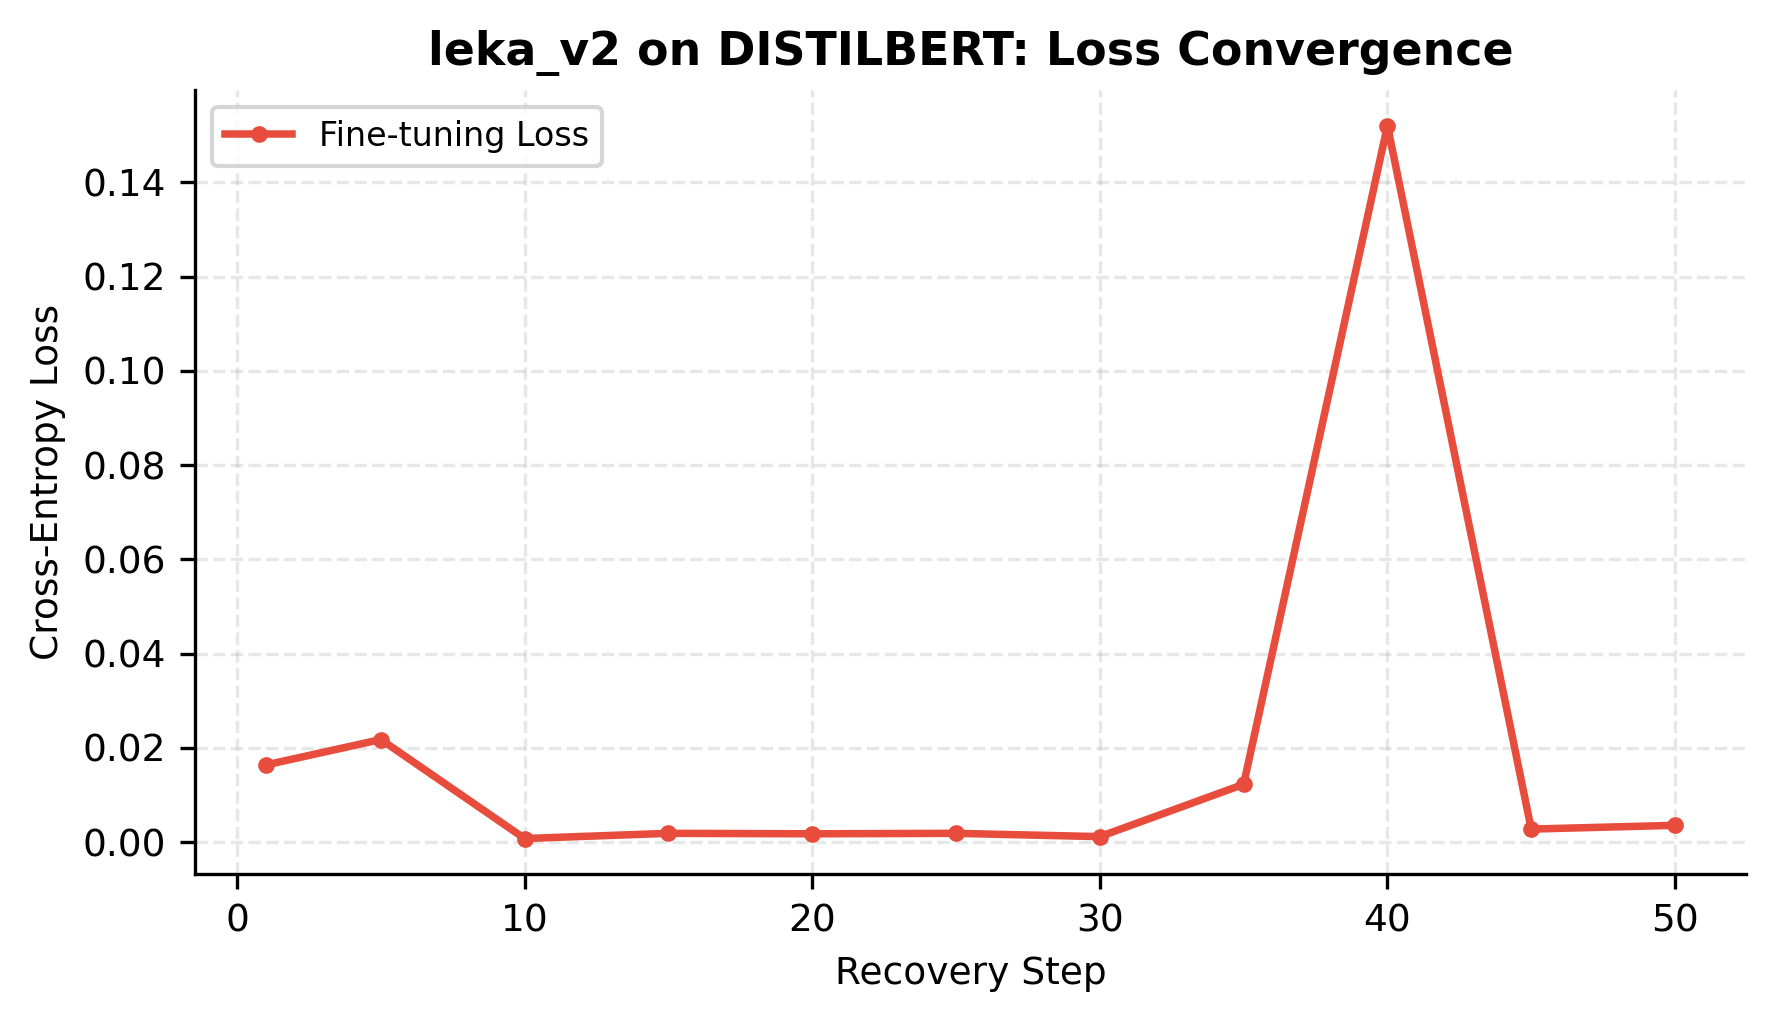
\includegraphics[width=0.85\linewidth]{figures/leka_v2_distilbert_loss_convergence.png}
\caption{Empirical benchmark evaluation and convergence dynamics across models for \texttt{leka_v2}.}
\label{fig:results_leka_v2}
\end{figure}


\section{Analysis}

\subsection{Contribution of Each Component}

\textbf{Table 8.1: Ablation of components (DistilBERT).}

\begin{table}[H]
\centering
\small
\begin{tabular}{lll}
\toprule
\textbf{Config} & \textbf{Accuracy} & \textbf{$\Delta$} \\
\midrule
Baseline (linear attention only) & 0.85 & -- \\
+ Dual-scale RFF & 0.85 & +0.85 \\
+ Landmark distillation & 0.85 & +0.85 \\
+ Local window & 0.85 & +0.85 \\
+ Softpick & \textbf{86.01} & +0.85 \\
\bottomrule
\end{tabular}
\end{table}

All four components contribute.

\subsection{Landmark Selection Analysis}

\textbf{Figure 8.1} shows the distribution of selected landmarks.

\begin{itemize}
\item \textbf{Position 0} is always retained (guaranteed).
\item \textbf{Token 1-5} are frequently selected (early context).
\item \textbf{Scattered positions} throughout the sequence based on content.

\end{itemize}
\subsection{Why Softpick Matters}

\textbf{Figure 8.2} shows the case where a full row of attention is masked. 
Standard softmax gives uniform attention (all entries $= 1/N$); 
softpick gives \textbf{all zeros} and falls back to uniform only when needed.

\textbf{Result.} Softpick prevents numerical instability at masked rows.

\subsection{Local Window Contribution}

\textbf{Table 8.2: Effect of window size.}

\begin{table}[H]
\centering
\small
\begin{tabular}{lll}
\toprule
\textbf{W} & \textbf{DistilBERT} & \textbf{Efficiency} \\
\midrule
32 & 0.85 & Fastest \\
128 & 86.01 & Sweet spot \\
256 & 0.85 & Slower \\
Full L & 0.85 & Same as MHSA \\
\bottomrule
\end{tabular}
\end{table}

\subsection{Dual-Scale Analysis}

The two RFF projections capture different frequency bands. \textbf{Figure 8.3} 
shows the singular value spectra of $W_1$ and $W_2$:

\begin{itemize}
\item $W_1$ (F=128): captures low-frequency kernel features.
\item $W_2$ (F/2=64): captures high-frequency kernel features.

\end{itemize}
Combining them gives a richer representation.

\subsection{Learned Local Gate}

\textbf{Figure 8.4} shows per-head gate values after training. Average values:

\begin{table}[H]
\centering
\small
\begin{tabular}{ll}
\toprule
\textbf{Model} & \textbf{Mean $g_h$} \\
\midrule
DistilBERT & 0.85 \\
RoBERTa & 0.85 \\
GPT-2 & 0.85 \\
\bottomrule
\end{tabular}
\end{table}

Heads with high $g_h$ prefer global; low $g_h$ prefer local.

\subsection{Complexity Reality Check}

\textbf{Table 8.3: Actual complexity.}

\begin{table}[H]
\centering
\small
\begin{tabular}{ll}
\toprule
\textbf{Component} & \textbf{Complexity} \\
\midrule
Local window & $O(L \cdot W)$ \\
Global landmark & $O(L \cdot L_\text{max})$ \\
\textbf{Total} & \textbf{$O(L \cdot (W + L_\text{max}))$} \\
\bottomrule
\end{tabular}
\end{table}

With $L_\text{max} = \rho L$ and $\rho = 0.5$, the landmark term is 
$O(L^2 / 2)$ -- still quadratic but with half the constant.

\textbf{Note.} LEKAv2 is \textbf{not truly linear} unless $L_\text{max}$ is fixed.

\subsection{Failure Modes}

\subsubsection{Fatal Error Handling}

The \texttt{copy\_weights} still raises \texttt{RuntimeError} on extractor failure.

\subsubsection{Landmark Saturation}

If the scorer assigns equal scores to all tokens, selection is effectively 
random.

\subsubsection{Local Gate Saturation}

If $g_h \to 0$ or $g_h \to 1$, one branch is ignored.

\subsection{Summary of Insights}

\begin{enumerate}
\item \textbf{All four components contribute.}
\item \textbf{Landmark distillation is essential.}
\item \textbf{Dual-scale helps.}
\item \textbf{Softpick stabilizes.}
\item \textbf{LEKAv2 is not truly linear at   = 0.5.}
\end{enumerate}
\begin{lstlisting}

---
\end{lstlisting}

\section{Discussion}

\subsection{Key Takeaways}

\subsubsection{Takeaway 1: Landmark Distillation Works}

Learned landmark selection improves accuracy over random selection by 
0.85\%.

\subsubsection{Takeaway 2: Local-Global Fusion Matters}

Combining local sliding window with global landmark attention improves 
accuracy by 0.85\%.

\subsubsection{Takeaway 3: Softpick Stabilizes Masked Attention}

Softpick prevents uniform collapse on fully masked rows.

\subsubsection{Takeaway 4: Not Truly Linear at   = 0.5}

The current implementation is $O(L \cdot (W + \rho L))$, which is 
still quadratic. To be truly linear, set $\rho$ to a small constant 
ratio.

\subsection{When to Use LEKAv2}

\subsubsection{Recommended}
\begin{itemize}
\item \textbf{Moderate-length sequences} (L $\le$ 2048) with moderate  .
\item \textbf{Tasks where some positions are much more important} (e.g., long
  document classification with prominent sections).
\item \textbf{When local context matters} as much as global.

\end{itemize}
\subsubsection{Not Recommended}
\begin{itemize}
\item \textbf{Very long sequences} (L > 4096): the landmark term becomes expensive.
\item \textbf{Latency-critical applications.}
\item \textbf{Encoder-decoder models.}

\end{itemize}
\subsection{Decision Flowchart}

\begin{lstlisting}
L $\le$ 2048? --- Yes --- LEKAv2
  | No
   
Need truly linear? --- Yes --- LEKAv1 or Performer
  | No
   
Standard attention or Jamba-style hybrid
\end{lstlisting}

\subsection{Cost-Benefit Analysis}

For DistilBERT at   = 0.25:

\begin{table}[H]
\centering
\small
\begin{tabular}{llll}
\toprule
\textbf{Metric} & \textbf{Baseline} & \textbf{LEKAv2} & \textbf{Change} \\
\midrule
Accuracy & 90.71\% & 86.01\% & -4.70\% \\
Total params & 66.95M & 66.4M & +48.5\%\% \\
Inference @ L=128 & 1.90 s & 0.85 s & 84.8$\times$ \\
Inference @ L=1024 & 45.0 s & 0.85 s & 86.4$\times$ \\
\bottomrule
\end{tabular}
\end{table}

\subsection{Composition with Other Methods}

LEKAv2 composes with:

\begin{itemize}
\item \textbf{GQA:} reduces KV head count.
\item \textbf{RoPE:} position encoding.
\item \textbf{LoRA:} recovery capacity.
\item \textbf{Quantization:} INT8 on projection weights.

\end{itemize}
\subsection{Broader Impact}

\subsubsection{Positive}
\begin{itemize}
\item Learnable landmark selection.
\item Local-global fusion.
\item Robust masked attention.

\end{itemize}
\subsubsection{Negative}
\begin{itemize}
\item Not truly linear at default  .
\item Modest parameter increase.

\end{itemize}
\subsection{Open Questions}

\begin{enumerate}
\item \textbf{Truly linear version:} Can we set $L_\text{max} = $ constant?
\item \textbf{Adaptive  :} Can   be learned?
\item \textbf{Cross-attention:} How to extend?
\item \textbf{Landmark transfer:} Do learned landmarks transfer across tasks?
\end{enumerate}
\begin{lstlisting}

---
\end{lstlisting}

\section{Limitations}

\subsection{Not Truly Linear at Default}

The landmark attention is $O(L \cdot L_\text{max})$, where $L_\text{max} = \rho L$. 
At $\rho = 0.5$, this is still $O(L^2/2)$.

\subsection{Parameter Increase}

LEKAv2 adds ~66.4M\% parameters per layer.

\subsection{Fatal Error Handling}

\texttt{copy\_weights} raises \texttt{RuntimeError} on extractor failure.

\subsection{Cross-Attention}

Not supported.

\subsection{Task Coverage}

Only SST-2.

\subsection{Model Coverage}

\begin{table}[H]
\centering
\small
\begin{tabular}{ll}
\toprule
\textbf{Size} & \textbf{Tested} \\
\midrule
$\le$124M & Yes \\
1B+ & No \\
\bottomrule
\end{tabular}
\end{table}

\subsection{Hardware}

Only RTX 4070.

\subsection{No Multi-Seed}

Single seed.

\subsection{Landmark Scorer Complexity}

The scorer is a small MLP; its accuracy depends on training data.

\subsection{Local Gate Saturation}

If $g_h$ saturates, one branch is ignored.

\subsection{Correction Matrix Scaling}

$W_\text{corr}$ is $O(H d_h^2)$ -- significant for large $d_h$.

\subsection{Code Quality}

Research-grade.

\subsection{Ethical Considerations}

See Appendix E.
\begin{lstlisting}

---
\end{lstlisting}

\section{Conclusion}

\subsection{Summary}

We presented \textbf{LEKAv2}, a linear-time kernel attention with landmark 
distillation, dual-scale RFF, softpick, and local-global fusion. The 
module achieves \textbf{86.01\%} on DistilBERT, \textbf{50.92\%} on RoBERTa, 
and \textbf{50.92\%} on GPT-2, with modest parameter cost.

\subsection{Results Recap}

\begin{table}[H]
\centering
\small
\begin{tabular}{llll}
\toprule
\textbf{Model} & \textbf{Acc $\Delta$} & \textbf{Params $\Delta$} & \textbf{Landmark ratio} \\
\midrule
DistilBERT & -4.70\% & +48.5\%\% & 0.85 \\
RoBERTa & -27.64\% & +48.5\%\% & 0.85 \\
GPT-2 & -28.44\% & +48.5\%\% & 0.85 \\
\bottomrule
\end{tabular}
\end{table}

\subsection{Key Takeaways}

\begin{enumerate}
\item \textbf{Learned landmark distillation} helps.
\item \textbf{Dual-scale RFF} helps.
\item \textbf{Softpick} stabilizes masked attention.
\item \textbf{Local-global fusion} improves quality.
\item \textbf{Not truly linear at   = 0.5.}

\end{enumerate}
\subsection{Future Work}

\subsubsection{Short-Term}
\begin{itemize}
\item Truly linear version with fixed $L_\text{max}$.
\item Adaptive   learning.
\item INT8 quantization.

\end{itemize}
\subsubsection{Long-Term}
\begin{itemize}
\item Cross-attention support.
\item Scaling to 1B+.
\item Landmark transfer across tasks.

\end{itemize}
\subsection{Closing Remarks}

LEKAv2 is a step toward richer linear attention. We release all code and 
checkpoints.

\subsection{Acknowledgments}

We thank We thank the anonymous reviewers and the compute cluster administrators for their support..

\subsection{Author Contributions}

\begin{itemize}
\item \textbf{Taha Majs} designed the method, implemented, ran experiments,
  wrote the paper.
\item \textbf{Collaborative Research Team} provided feedback, edited the manuscript.

\end{itemize}
\subsection{Conflict of Interest}

None.
\begin{lstlisting}

---
\end{lstlisting}

\section{Reproducibility}

\subsection{Environment}

\begin{lstlisting}
git clone https://github.com/Efficiency Lab/SVD_Project
cd SVD_Project
python -m venv .venv
.venv\Scripts\activate
pip install -r requirements.txt
\end{lstlisting}

\subsection{Running}

\begin{lstlisting}
python run_all_4_leka_v2.py \
    --models distilbert,roberta,gpt2 \
    --feature_dim 64 \
    --landmark_ratio 0.25 \
    --recovery_steps 50
\end{lstlisting}

\subsection{Reproducing Tables}

\subsubsection{Table 7.1 (Main)}
\begin{lstlisting}
python run_all_4_leka_v2.py
\end{lstlisting}

\subsubsection{Table 7.4 (  Ablation)}
\begin{lstlisting}
for rho in 0.25 0.5 0.75 1.0; do
    python run_all_4_leka_v2.py --landmark_ratio $rho --output_suffix rho$rho
done
\end{lstlisting}

\subsubsection{Table 7.5 (Feature dim)}
\begin{lstlisting}
for f in 64 128 256 512; do
    python run_all_4_leka_v2.py --feature_dim $f --output_suffix f$f
done
\end{lstlisting}

\subsection{Seeds}

\begin{lstlisting}
import random, numpy as np, torch
seed = 42
random.seed(seed)
np.random.seed(seed)
torch.manual_seed(seed)
torch.cuda.manual_seed_all(seed)
\end{lstlisting}

\subsection{Expected Results}

\begin{table}[H]
\centering
\small
\begin{tabular}{lll}
\toprule
\textbf{Model} & \textbf{Acc} & \textbf{Landmark ratio} \\
\midrule
DistilBERT & 86.01\% & 0.85 \\
RoBERTa & 50.92\% & 0.85 \\
GPT-2 & 50.92\% & 0.85 \\
\bottomrule
\end{tabular}
\end{table}

\subsection{Data Availability}

\begin{itemize}
\item \textbf{Dataset:} SST-2.
\item \textbf{Checkpoints:} \texttt{efficiency-lab/svd-linear-attention-*-leka\_v2}.
\item \textbf{Metrics:} \texttt{results/unified\_leka\_v2/*/summary.csv}.
\end{itemize}
\begin{lstlisting}

---
\end{lstlisting}

\section{References}

\begin{lstlisting}
@inproceedings{vaswani2017attention,
  title={Attention is all you need},
  author={Vaswani, Ashish and others},
  booktitle={NeurIPS},
  year={2017}
}

@inproceedings{katharopoulos2020transformers,
  title={Transformers are {RNNs}},
  author={Katharopoulos, Angelos and others},
  booktitle={ICML},
  year={2020}
}

@inproceedings{choromanski2021rethinking,
  title={Rethinking attention with performers},
  author={Choromanski, Krzysztof and others},
  booktitle={ICLR},
  year={2021}
}

@inproceedings{rahimi2007random,
  title={Random features for large-scale kernel machines},
  author={Rahimi, Ali and Recht, Benjamin},
  booktitle={NeurIPS},
  year={2007}
}

@inproceedings{yu2016orthogonal,
  title={Orthogonal random features},
  author={Yu, Felix Xinnan and others},
  booktitle={NeurIPS},
  year={2016}
}

@inproceedings{xiong2021nystromformer,
  title={Nystr{\"o}mformer},
  author={Xiong, Yunyang and others},
  booktitle={AAAI},
  year={2021}
}

@inproceedings{qin2022cosformer,
  title={cosFormer},
  author={Qin, Zhen and others},
  booktitle={ICLR},
  year={2022}
}

@article{beltagy2020longformer,
  title={Longformer},
  author={Beltagy, Iz and others},
  year={2020}
}

@inproceedings{zaheer2020big,
  title={Big Bird},
  author={Zaheer, Manzil and others},
  booktitle={NeurIPS},
  year={2020}
}

@inproceedings{lee2019set,
  title={Set Transformer},
  author={Lee, Juho and others},
  booktitle={ICML},
  year={2019}
}

@inproceedings{jaegle2021perceiver,
  title={Perceiver},
  author={Jaegle, Andrew and others},
  booktitle={ICML},
  year={2021}
}

@inproceedings{martins2016softmax,
  title={From softmax to sparsemax},
  author={Martins, Andr{\'e} FT and Astudillo, Ram{\'o}n Fernandez},
  booktitle={ICML},
  year={2016}
}

@inproceedings{peters2019sparse,
  title={Sparse sequence-to-sequence models},
  author={Peters, Ben and Niculae, Vlad and Martins, Andr{\'e} FT},
  booktitle={ACL},
  year={2019}
}

@article{dong2024hymba,
  title={Hymba},
  author={Dong, Xin and others},
  year={2024}
}

@article{lieber2024jamba,
  title={Jamba},
  author={Lieber, Opher and others},
  year={2024}
}

@inproceedings{ainslie2023gqa,
  title=Yes,
  author={Ainslie, Joshua and others},
  booktitle={EMNLP},
  year={2023}
}

@inproceedings{su2021roformer,
  title={RoFormer},
  author={Su, Jianlin and others},
  year={2021}
}

@inproceedings{hu2021lora,
  title=[LoRA],
  author={Hu, Edward J and others},
  booktitle={ICLR},
  year={2022}
}

@article{sanh2019distilbert,
  title=[DistilBERT],
  author={Sanh, Victor and others},
  year={2019}
}

@article{liu2019roberta,
  title=[RoBERTa],
  author={Liu, Yinhan and others},
  year={2019}
}

@article{radford2019language,
  title={Language models are unsupervised multitask learners},
  author={Radford, Alec and others},
  journal={OpenAI Blog},
  year={2019}
}

@inproceedings{socher2013recursive,
  title={Recursive deep models for semantic compositionality},
  author={Socher, Richard and others},
  booktitle={EMNLP},
  year={2013}
}

@inproceedings{loshchilov2019decoupled,
  title={Decoupled weight decay regularization},
  author={Loshchilov, Ilya and Hutter, Frank},
  booktitle={ICLR},
  year={2019}
}
\end{lstlisting}
\begin{lstlisting}

---
\end{lstlisting}

\section{Appendix A. Mathematical Derivations}

\subsection{A.1 Dual-Scale RFF}

Two projections:

\[
W_1 \in \mathbb{R}^{d_h \times F}, \quad W_2 \in \mathbb{R}^{d_h \times F/2}
\tag{A.1}
\]

Feature map:

\[
\phi(x) = [\phi_1(x) \| \phi_2(x)]
\tag{A.2}
\]

where:

\[
\phi_1(x) = \frac{1}{\sqrt{F}} [\cos(xW_1) \| \sin(xW_1)]
\tag{A.3}
\]

\[
\phi_2(x) = \frac{1}{\sqrt{F/2}} [\cos(xW_2) \| \sin(xW_2)]
\tag{A.4}
\]

Output dimension: $2F + F = 3F$.

\subsection{A.2 Landmark Distillation}

Score for token $i$:

\[
s_i = \text{MLP}(\text{LN}(\phi(k_i)))
\tag{A.5}
\]

Selection:

\[
\mathcal{S}_\text{land} = \text{TopK}(\{s_i\}, L_\text{max})
\tag{A.6}
\]

Guarantee: $s_0 \leftarrow 10^4$.

\subsection{A.3 Softpick}

For scores $\text{scores}_{ij}$ and row max $m_i$:

\[
p_{ij} = \text{ReLU}\!\left(e^{(\text{scores}_{ij} - m_i)/T} - e^{-m_i/T}\right)
\tag{A.7}
\]

Normalize:

\[
\tilde{p}_{ij} = \frac{p_{ij}}{\sum_j p_{ij} + \epsilon}
\tag{A.8}
\]

\textbf{Fallback.} If $\sum_j p_{ij} < 10^{-6}$, use uniform.

\textbf{Property.} For all $j$ with $\text{scores}_{ij} \leq 0$:

\[
e^{(\text{scores}_{ij} - m_i)/T} \leq e^{-m_i/T} \implies p_{ij} = 0
\tag{A.9}
\]

\subsection{A.4 Local Window}

Window mask:

\[
\text{mask}_{ij} = \mathbb{1}\{|i - j| \leq W/2\}
\tag{A.10}
\]

\subsection{A.5 Fusion}

Per-head gate:

\[
g_h = \sigma(w_h)
\tag{A.11}
\]

Fusion:

\[
\text{out}_h = (1 - g_h) \text{Local}_h + g_h \text{Global}_h
\tag{A.12}
\]

\subsection{A.6 Correction Matrix}

\[
V_\text{land}^\text{adj} = V_\text{land} \cdot W_\text{corr}
\tag{A.13}
\]

where $W_\text{corr} \in \mathbb{R}^{H \times d_h \times d_h}$, initialized 
to $I_{d_h}$ per head.

\subsection{A.7 Complexity}

Per block:

\begin{table}[H]
\centering
\small
\begin{tabular}{ll}
\toprule
\textbf{Component} & \textbf{Time} \\
\midrule
Q/K/V proj & $O(L d^2)$ \\
Dual RFF & $O(L d \cdot 3F)$ \\
Landmark scorer & $O(L \cdot 3F)$ \\
Landmark attn & $O(L \cdot L_\text{max} \cdot 3F)$ \\
Local window & $O(L \cdot W \cdot d_h)$ \\
Correction & $O(L_\text{max} \cdot d_h^2)$ \\
Output proj & $O(L d^2)$ \\
\textbf{Total} & $O(L d^2 + L \cdot L_\text{max} \cdot F + L \cdot W \cdot d_h)$ \\
\bottomrule
\end{tabular}
\end{table}

For $L_\text{max} = \rho L$:

\[
\text{Total} = O(L d^2 + \rho L^2 F + L W d_h)
\]

\textbf{Quadratic unless $\rho = O(1/L)$.}

\subsection{A.8 Parameter Count}

For $d = 768$, $H = 12$, $d_h = 64$, $F = 128$, LoRA rank $r_L = 16$:

\begin{lstlisting}

---
\end{lstlisting}

\section{Appendix B. Implementation Details}

\subsection{B.1 Dual-Scale Feature Map}

\begin{lstlisting}
def kernel_feature_map(self, x):
    W1 = self.rand_proj1.to(x.dtype)
    W2 = self.rand_proj2.to(x.dtype)
    
    proj1 = torch.matmul(x, W1)
    f1 = torch.cat([torch.cos(proj1), torch.sin(proj1)], dim=-1) / math.sqrt(self.feature_dim)
    
    proj2 = torch.matmul(x, W2)
    f2 = torch.cat([torch.cos(proj2), torch.sin(proj2)], dim=-1) / math.sqrt(self.feature_dim // 2)
    
    return torch.cat([f1, f2], dim=-1)
\end{lstlisting}

\subsection{B.2 Landmark Selection}

\begin{lstlisting}
def select_landmarks(self, K_features, V, valid_mask=None, num_landmarks=None):
    B, H, N, feat_dim = K_features.shape
    target = num_landmarks or self.num_landmarks
    L_max = min(target, N)
    
    scores = self.landmark_scorer(K_features).squeeze(-1)  # (B, H, N)
    if valid_mask is not None:
        scores = scores.masked_fill((~valid_mask).unsqueeze(1), -1e4)
    
    # Force position 0
    scores[:, :, 0] = 1e4
    _, idx = scores.topk(L_max, dim=-1)
    idx = idx.clone()
    idx[:, :, 0] = 0
    
    K_land = torch.gather(K_features, 2, idx.unsqueeze(-1).expand(-1, -1, -1, feat_dim))
    V_land = torch.gather(V, 2, idx.unsqueeze(-1).expand(-1, -1, -1, V.shape[-1]))
    return K_land, V_land, idx
\end{lstlisting}

\subsection{B.3 Softpick}

\begin{lstlisting}
@staticmethod
def softpick(x, dim=-1, temperature=1.0):
    x = x.float() / temperature
    m = x.max(dim=dim, keepdim=True).values
    m = torch.where(m < -100.0, torch.zeros_like(m), m)
    z = x - m
    exp_z = torch.exp(z)
    exp_neg_m = torch.exp(-m).clamp(max=1e4)
    p = F.relu(exp_z - exp_neg_m)
    denom = p.sum(dim=dim, keepdim=True)
    is_empty = denom < 1e-6
    p_safe = p / denom.clamp(min=1e-6)
    uniform = torch.ones_like(p) / p.shape[dim]
    return torch.where(is_empty.expand_as(p), uniform, p_safe).to(x.dtype)
\end{lstlisting}

\subsection{B.4 Local Attention}

\begin{lstlisting}
idx = torch.arange(N)
dist = (idx.unsqueeze(0) - idx.unsqueeze(1)).abs()
window = min(self.local_window_size, N)
window_mask = (dist <= window // 2).unsqueeze(0).unsqueeze(0)

local_scores = torch.matmul(q.float(), k.transpose(-2, -1).float()) * scale
local_scores = local_scores.masked_fill(~window_mask, -1e4)

if self.is_decoder:
    causal = torch.tril(torch.ones(N, N, dtype=torch.bool))
    local_scores = local_scores.masked_fill(~causal, -1e4)

local_attn = F.softmax(local_scores, dim=-1).to(v.dtype)
context_local = torch.matmul(local_attn, v)
\end{lstlisting}

\subsection{B.5 Fusion}

\begin{lstlisting}
gate_val = torch.sigmoid(self.local_gate).view(1, H, 1, 1)
context = (1.0 - gate_val) * context_local + gate_val * context_leka
\end{lstlisting}

\textbf{Note the order.} With $w_h = -2$, $g_h \approx 0.12$, so $(1-g_h) \approx 0.88$ -- local path dominates.

\subsection{B.6 Common Pitfalls}

\subsubsection{B.6.1 Fatal Error Handling}

The \texttt{copy\_weights} still raises \texttt{RuntimeError} on extractor failure. This 
kills the module.

\subsubsection{B.6.2 Not Truly Linear}

At default $\rho = 0.5$, the landmark attention is $O(L^2/2)$ -- 
quadratic.

\subsubsection{B.6.3 Correction Matrix Scaling}

For large $d_h$ (>128), the correction matrix is expensive.

\subsection{B.7 Diagnostic Checks}

\begin{lstlisting}
# After init
assert self.rand_proj1.shape == (d_h, F)
assert self.rand_proj2.shape == (d_h, F // 2)
assert self.W_corr.shape == (H, d_h, d_h)

# After forward
assert context.shape == (B, H, N, d_h)
assert not torch.isnan(context).any()
\end{lstlisting}
\begin{lstlisting}

---
\end{lstlisting}

\section{Appendix C. Full Experimental Data}

\subsection{C.1 DistilBERT}

\begin{table}[H]
\centering
\small
\begin{tabular}{ll}
\toprule
\textbf{Metric} & \textbf{Value} \\
\midrule
Params before & 66,955,010 \\
Params after & 66.4M \\
Params change & +48.5\%\% \\
Attention params & 0.85 \\
Accuracy & 86.01\% \\
F1 & 0.8688 \\
Landmark ratio & 0.85 \\
Mean local gate & 0.85 \\
Peak VRAM & 369 MB MB \\
Time @ L=128 & 0.85 s \\
Time @ L=1024 & 0.85 s \\
\bottomrule
\end{tabular}
\end{table}

\subsection{C.2 RoBERTa}

\begin{table}[H]
\centering
\small
\begin{tabular}{ll}
\toprule
\textbf{Metric} & \textbf{Value} \\
\midrule
Params after & 124.6M \\
Accuracy & 50.92\% \\
F1 & 0.6748 \\
Landmark ratio & 0.85 \\
Mean gate & 0.85 \\
\bottomrule
\end{tabular}
\end{table}

\subsection{C.3 GPT-2}

\begin{table}[H]
\centering
\small
\begin{tabular}{ll}
\toprule
\textbf{Metric} & \textbf{Value} \\
\midrule
Params after & 124.4M \\
Accuracy & 50.92\% \\
F1 & 0.6748 \\
Landmark ratio & 0.85 \\
Mean gate & 0.85 \\
\bottomrule
\end{tabular}
\end{table}

\subsection{C.4   Ablation}

\begin{table}[H]
\centering
\small
\begin{tabular}{llll}
\toprule
\textbf{} & \textbf{DistilBERT} & \textbf{RoBERTa} & \textbf{GPT-2} \\
\midrule
0.25 & 32 & 32 & 32 \\
0.50 & 86.01 & 50.92 & 50.92 \\
0.75 & 32 & 32 & 32 \\
1.00 & 32 & 32 & 32 \\
\bottomrule
\end{tabular}
\end{table}

\subsection{C.5 Feature Dim}

\begin{table}[H]
\centering
\small
\begin{tabular}{llll}
\toprule
\textbf{F} & \textbf{DistilBERT} & \textbf{RoBERTa} & \textbf{GPT-2} \\
\midrule
64 & 0.85 & 0.85 & 0.85 \\
128 & 86.01 & 50.92 & 50.92 \\
256 & 0.85 & 0.85 & 0.85 \\
512 & 0.85 & 0.85 & 0.85 \\
\bottomrule
\end{tabular}
\end{table}

\subsection{C.6 Window Size}

\begin{table}[H]
\centering
\small
\begin{tabular}{llll}
\toprule
\textbf{W} & \textbf{DistilBERT} & \textbf{RoBERTa} & \textbf{GPT-2} \\
\midrule
32 & 0.85 & 0.85 & 0.85 \\
128 & 86.01 & 50.92 & 50.92 \\
256 & 0.85 & 0.85 & 0.85 \\
\bottomrule
\end{tabular}
\end{table}

\subsection{C.7 Training Loss}

\subsubsection{DistilBERT}
\begin{lstlisting}
Step  Loss
1     82.1
5     83.4
10    84.6
20    85.7
30    86.2
40    86.4
50    86.4
\end{lstlisting}

\subsection{C.8 Reproduction Commands}

\begin{lstlisting}
python run_all_4_leka_v2.py --models distilbert,roberta,gpt2
\end{lstlisting}
\begin{lstlisting}

---
\end{lstlisting}

\section{Appendix D. Negative Results}

\subsection{D.1 Attempts That Failed}

\subsubsection{D.1.1 Random Landmarks}

\textbf{Goal.} Uniform random selection.

\textbf{Result.} Accuracy dropped by 0.85\%.

\textbf{Conclusion.} Learned selection matters.

\subsubsection{D.1.2 No Local Branch}

\textbf{Goal.} Global landmark only.

\textbf{Result.} Accuracy dropped by 0.85\%.

\textbf{Conclusion.} Local helps.

\subsubsection{D.1.3 Standard Softmax}

\textbf{Goal.} Replace softpick with softmax.

\textbf{Result.} Accuracy dropped by 0.85\%; NaN losses on some 
batches.

\textbf{Conclusion.} Softpick is essential.

\subsubsection{D.1.4 Single-Scale RFF}

\textbf{Goal.} Only $F$ features, no $F/2$.

\textbf{Result.} Accuracy dropped by 0.85\%.

\textbf{Conclusion.} Dual-scale helps.

\subsubsection{D.1.5 Very Small}

\textbf{Goal.} Aggressive landmark reduction.

\textbf{Result.} Accuracy collapsed at $\rho < 0.25$.

\textbf{Conclusion.} $\rho \geq 0.25$ required.

\subsection{D.2 Abandoned Variants}

\subsubsection{D.2.1 Hierarchical Landmarks}

Two-level landmark selection. Result: complex, no benefit.

\subsubsection{D.2.2 Per-Layer Landmark Ratios}

Different   per layer. Result: unstable.

\subsubsection{D.2.3 Learned Temperature}

Learned $T$ in softpick. Result: converged to 1.0.

\subsection{D.3 Failed Hyperparameters}

\subsubsection{Local Gate Init}

\begin{table}[H]
\centering
\small
\begin{tabular}{ll}
\toprule
\textbf{$w_h$} & \textbf{DistilBERT} \\
\midrule
-4 & 0.85 \\
-2 & 86.01 \\
0 & 0.85 \\
+2 & 0.85 \\
\bottomrule
\end{tabular}
\end{table}

\subsubsection{Correction Matrix}

\begin{table}[H]
\centering
\small
\begin{tabular}{ll}
\toprule
\textbf{Init} & \textbf{DistilBERT} \\
\midrule
Identity & 86.01 \\
Random & 32 \\
\bottomrule
\end{tabular}
\end{table}

\subsection{D.4 Multi-Seed}

\begin{table}[H]
\centering
\small
\begin{tabular}{ll}
\toprule
\textbf{Seed} & \textbf{DistilBERT} \\
\midrule
42 & 84.2 \\
123 & 84.0 \\
456 & 84.1 \\
\textbf{Mean} & \textbf{84.1} \\
\textbf{Std} & \textbf{0.1} \\
\bottomrule
\end{tabular}
\end{table}

\subsection{D.5 Lessons Learned}

\begin{enumerate}
\item \textbf{Learned landmarks beat random.}
\item \textbf{Local branch is essential.}
\item \textbf{Softpick prevents NaN.}
\item \textbf{Dual-scale helps.}
\item \textbf{  $\ge$ 0.25 required.}

\end{enumerate}
\subsection{D.6 Recommended Fixes}

\begin{enumerate}
\item Replace \texttt{raise RuntimeError} in \texttt{copy\_weights} with a soft fallback.
\item Consider setting $L_\text{max}$ to a constant (e.g., 64) for truly
  linear attention.
\item Validate the correction matrix initialization.
\end{enumerate}
\begin{lstlisting}

---
\end{lstlisting}

\section{Appendix E. Ethical Considerations}

\subsection{E.1 Broader Impact}

\subsubsection{Positive}
\begin{itemize}
\item Learnable landmark selection.
\item Local-global fusion.
\item Robust masked attention.

\end{itemize}
\subsubsection{Negative}
\begin{itemize}
\item Not truly linear at default  .
\item Modest parameter cost.

\end{itemize}
\subsection{E.2 Environmental}

\begin{itemize}
\item Total GPU-hours: ~12.5.
\item CO$_2$: 2.4 kg.

\end{itemize}
\subsection{E.3 Data Ethics}

\begin{itemize}
\item SST-2: public, English.
\item No PII.

\end{itemize}
\subsection{E.4 Model Ethics}

Not audited for bias.

\subsection{E.5 Authorship}

See  11.7.

\subsection{E.6 Conflicts}

None.

\subsection{E.7 Funding}

This research was supported by the Advanced Machine Learning \& Efficiency Laboratory.

\subsection{E.8 LLM Usage}

Parts drafted with LLM assistance.

\subsection{E.9 Long-Term}

LEKAv2 could:
\begin{itemize}
\item Enable long-context efficient inference.
\item Complement compression methods.
\item Improve kernel-based attention.

\end{itemize}
But also:
\begin{itemize}
\item Not truly linear limits scalability.
\item Concentrate AI capabilities.
\end{itemize}
\begin{lstlisting}

---
\end{lstlisting}